\documentclass{article}
\usepackage[utf8]{inputenc}
\usepackage{hyperref}
\usepackage{mathtools}
\usepackage{graphicx}
\usepackage{scrextend}
\usepackage{amssymb}
\usepackage{placeins}

\title{DT057A Project}
\author{Rasmus Holm(raho1501),\\Marcus Johansson(majo1412) \&\\Markus Fält(mafl1400)}
\date{June 2019}

\begin{document}

\maketitle

\section{Part I: PRNG and Random Variables} \label{part1}
  \subsection{LCG - Linear Congruential Generator}
    For this project we were tasked to create a LCG\footnote{Linear Congruential Generator}. 
    A LCG uses a recurrence relation to create pseudo random uniformly distributed values, see equation \ref{recrel} for the relation used.
    \begin{equation} \label{recrel}
      X_{n+1} = (aX_{n} + c)\ mod\ m
    \end{equation}
    This equation was then implemented in C++, this is contained in a file called \href{https://github.com/NoRines/simulerings_projekt/blob/master/lcg.h}{\emph{lcg.h}}.
    Using this LCG we were then tasked to generate 1000 values and then test our implementation against the ns-3::UniformRandomVariable generator. 
    To test our implementation we were provided with these paramaters:
    \begin{align*}
      a=13 \\
      m=100 \\
      c=1 \\
      seed=1
    \end{align*}
    With these parameters we then generated the 1000 values, and stored the results.
    We then used these same parameters in the ns-3::UniformRandomVariable generator, and stored the results.
    We then compared the results from our implementation against the ns-3::UniformRandomVariable generator and what we noticed is that our implementation is more cyclic\footnote{Constantly repeating.} than the ns-3 implementation. 
    Where our implementation cycles every 20 values or so using the provided parameters.
    With this in mind we then tried to find a set of parameters that gave us better results.
    What we found out is that if $m$ is prime or $m$ is coprime against $a$ we would get a less cyclic generation, rather we would get as many values as possible between 0 and the value $m$.
    So what we can conclude is that the LCG is reliant on the fact that
    \begin{equation}
      (p)\ mod\ n \neq 0,\ p = prime,\ n \in \mathbb{Z}_{+} ,\ n < p
    \end{equation}
    to generate a usable amount of primes.
    Likewise we can conclude that it is enough for $a$ and $m$ to be coprime, as this will give the same results.
    With this in mind we can propose a good scheme to use while choosing parameters, and that scheme will use the fact that:
    \begin{equation}
      m = 2^{x}\ and\ a = 2y+1 \implies m\ and\ a\ is\ coprime \\
    \end{equation}
    When we measured the time for both the ns-3 and our implementation we found that our implementation were much faster.
    The ns-3 implementation took about 1 minute and 7 seconds to generate 1 billion numbers and our implementation took about 18 seconds.
  \subsection{ITM - Inverse Transform Method}
  The solution we used was presented in the lectures and is called the inverse transform method.
  This can easily be implemented if the cumulative distribution function can be inverted.
  This is because:
  $$ F_{X}=Pr[X \leqslant x]=Pr[F(U) \leqslant x]=Pr[F^{-1}(F(U)) \leqslant F^{-1}(x)]= $$
  $$ Pr[U \leqslant F^{-1}(x)]=F^{-1}(x)\ Assuming\ U \sim Unif[0,1] $$
  This shows that if the inverse to the cumulative distribution function can be found then this function can be used to map an uniformly distributed value between 0 and 1 to follow the desired distribution.
  
  In the case of the exponential distribution the inverse can easily be found which is:
  $$ F^{-1}(u)=-\beta * ln(1-u) $$
  Since we are interested in the exponential distribution and we have the inverse to the cumulative distribution function the inverse transform method can very easily be implemented.
  
  \subsection{ns-3 Normal Distribution Implementation}
  In NS-3 they generate normal distributed values using a rejection method called Box-Muller. In NS-3 they generate normal random values by generating two uniform random values u1 and u2 on the range [0,1] and then use these to generate normal values by following the equations below:
  $$v1 = 2 * u1 - 1$$
  $$v2 = 2 * u2 - 1$$
  $$w = v1^2 + v2^2$$
  $$y = \sqrt{\frac{-2*log(w)}{w}}$$
  $$x1 = mean + v1 * y * \sqrt{variance}$$
  $$x2 = mean + v2 * y * \sqrt{variance}$$
  $$Where\ x1,\ x2 \subseteq N(mean,variance).$$
  
  This polar method that NS-3 uses is a faster rejection method than many ordinary rejection methods, given that you can generate uniform random values at a fast rate while not using trigonometric function. 
  \subsection{Comparison of implementations and distributions}
  The figures below are the result of the ns-3 generation and our generation.
  \begin{figure}[h!]
    \centering
    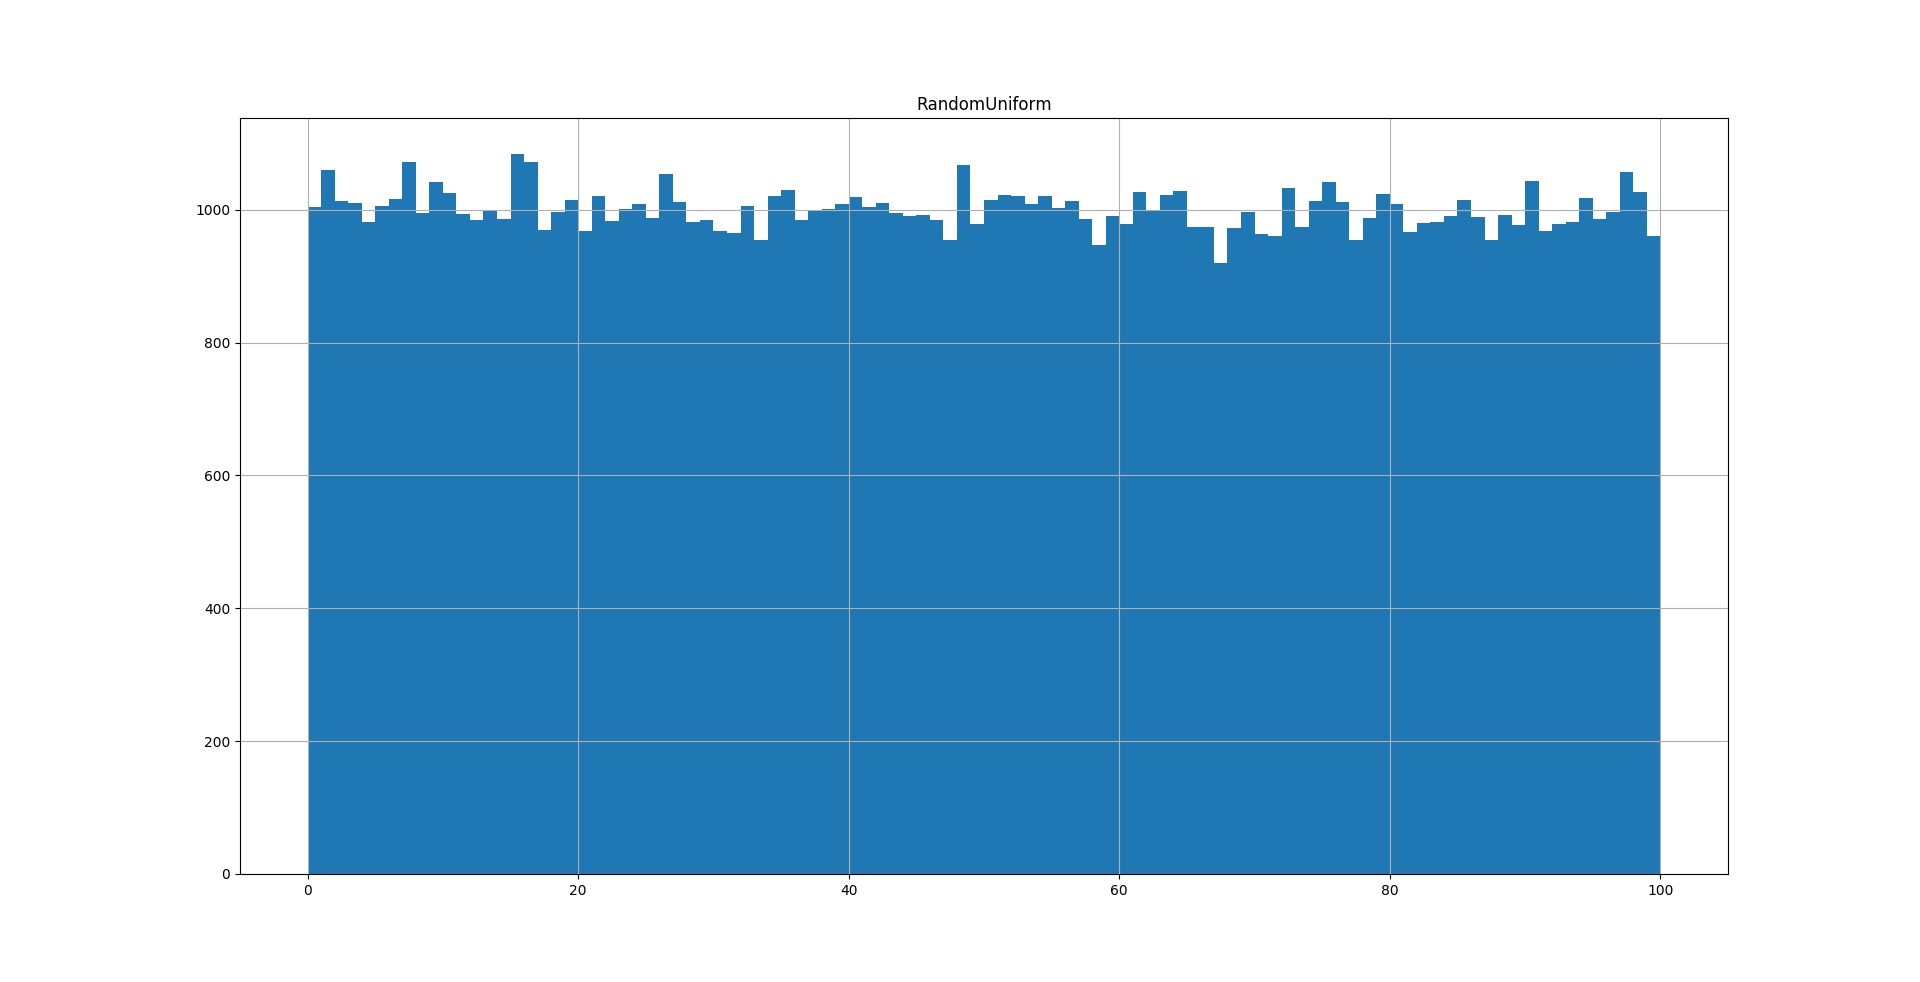
\includegraphics[width=\linewidth]{ns3uniform.png}
    \caption{ns3 RandomUniformVariable implementation.}
    \label{fig:ns-3ruv}
  \end{figure}
  
  \begin{figure}[h!]
    \centering
    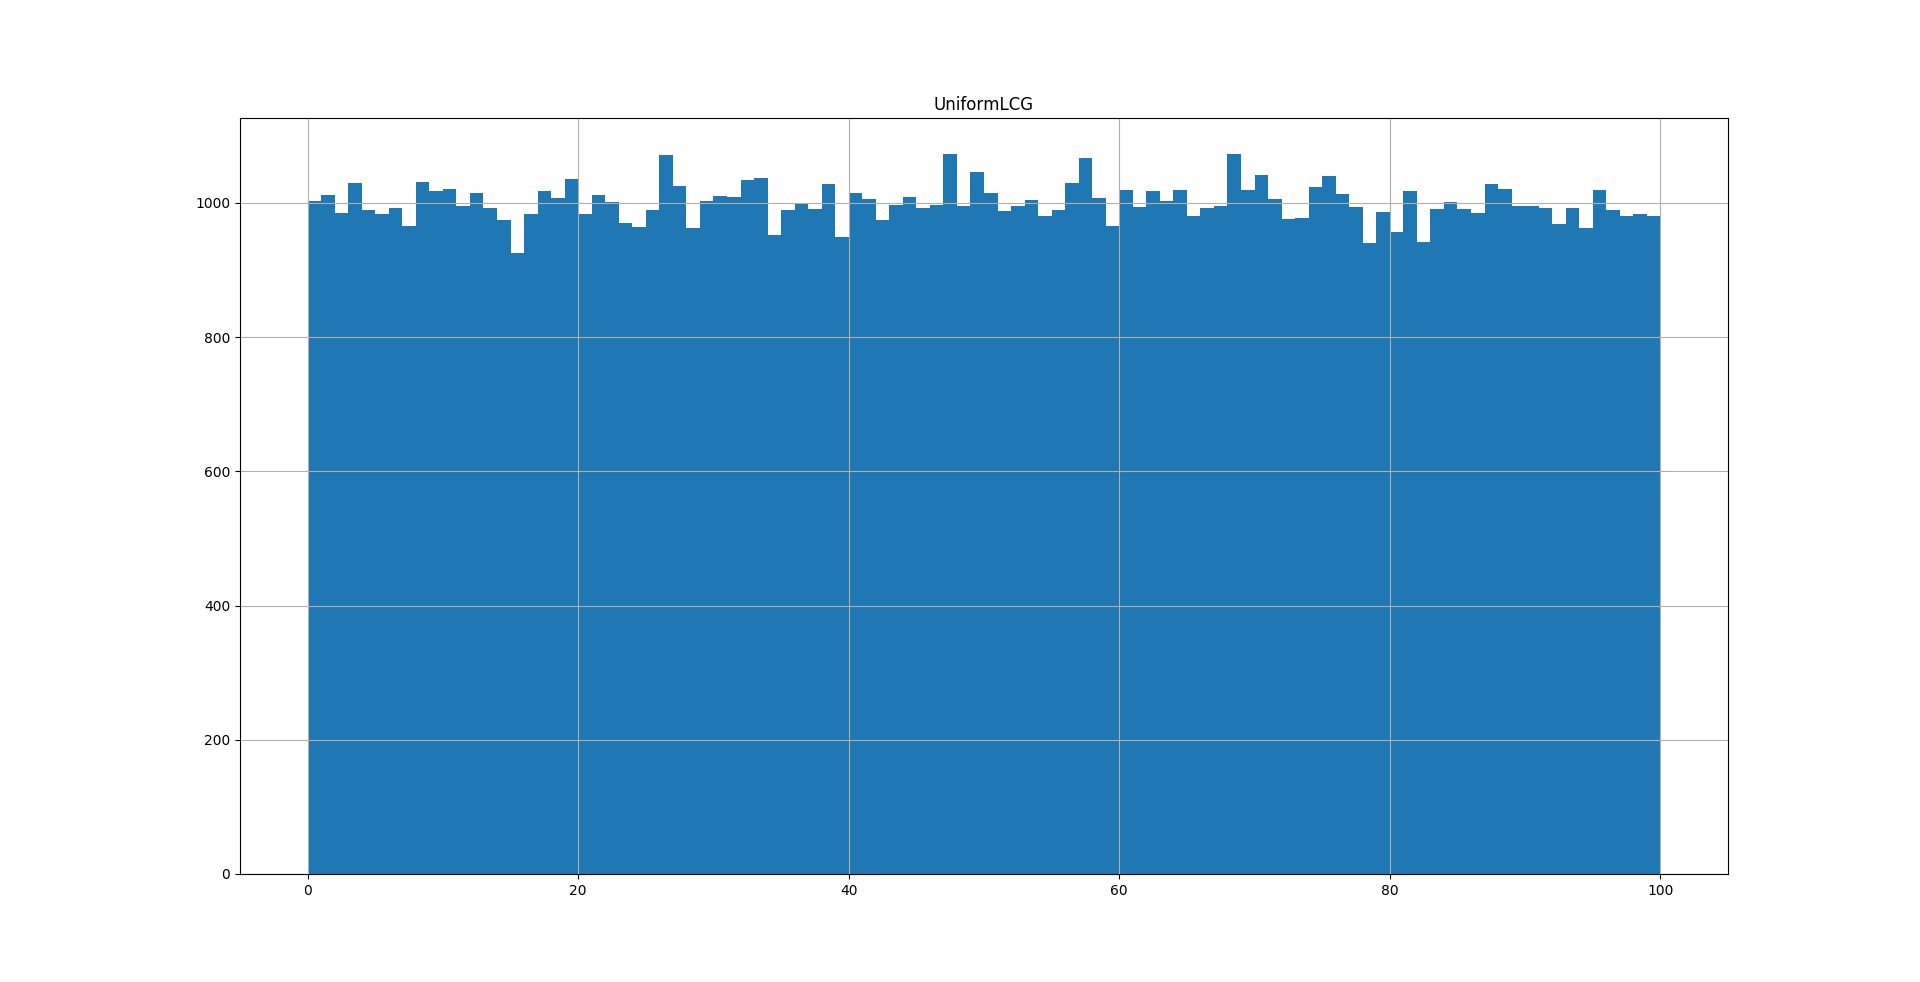
\includegraphics[width=\linewidth]{uniformLCG.png}
    \caption{LCG uniform random variable.}
    \label{fig:lcgruv}
  \end{figure}

  \begin{figure}[h!]
    \centering
      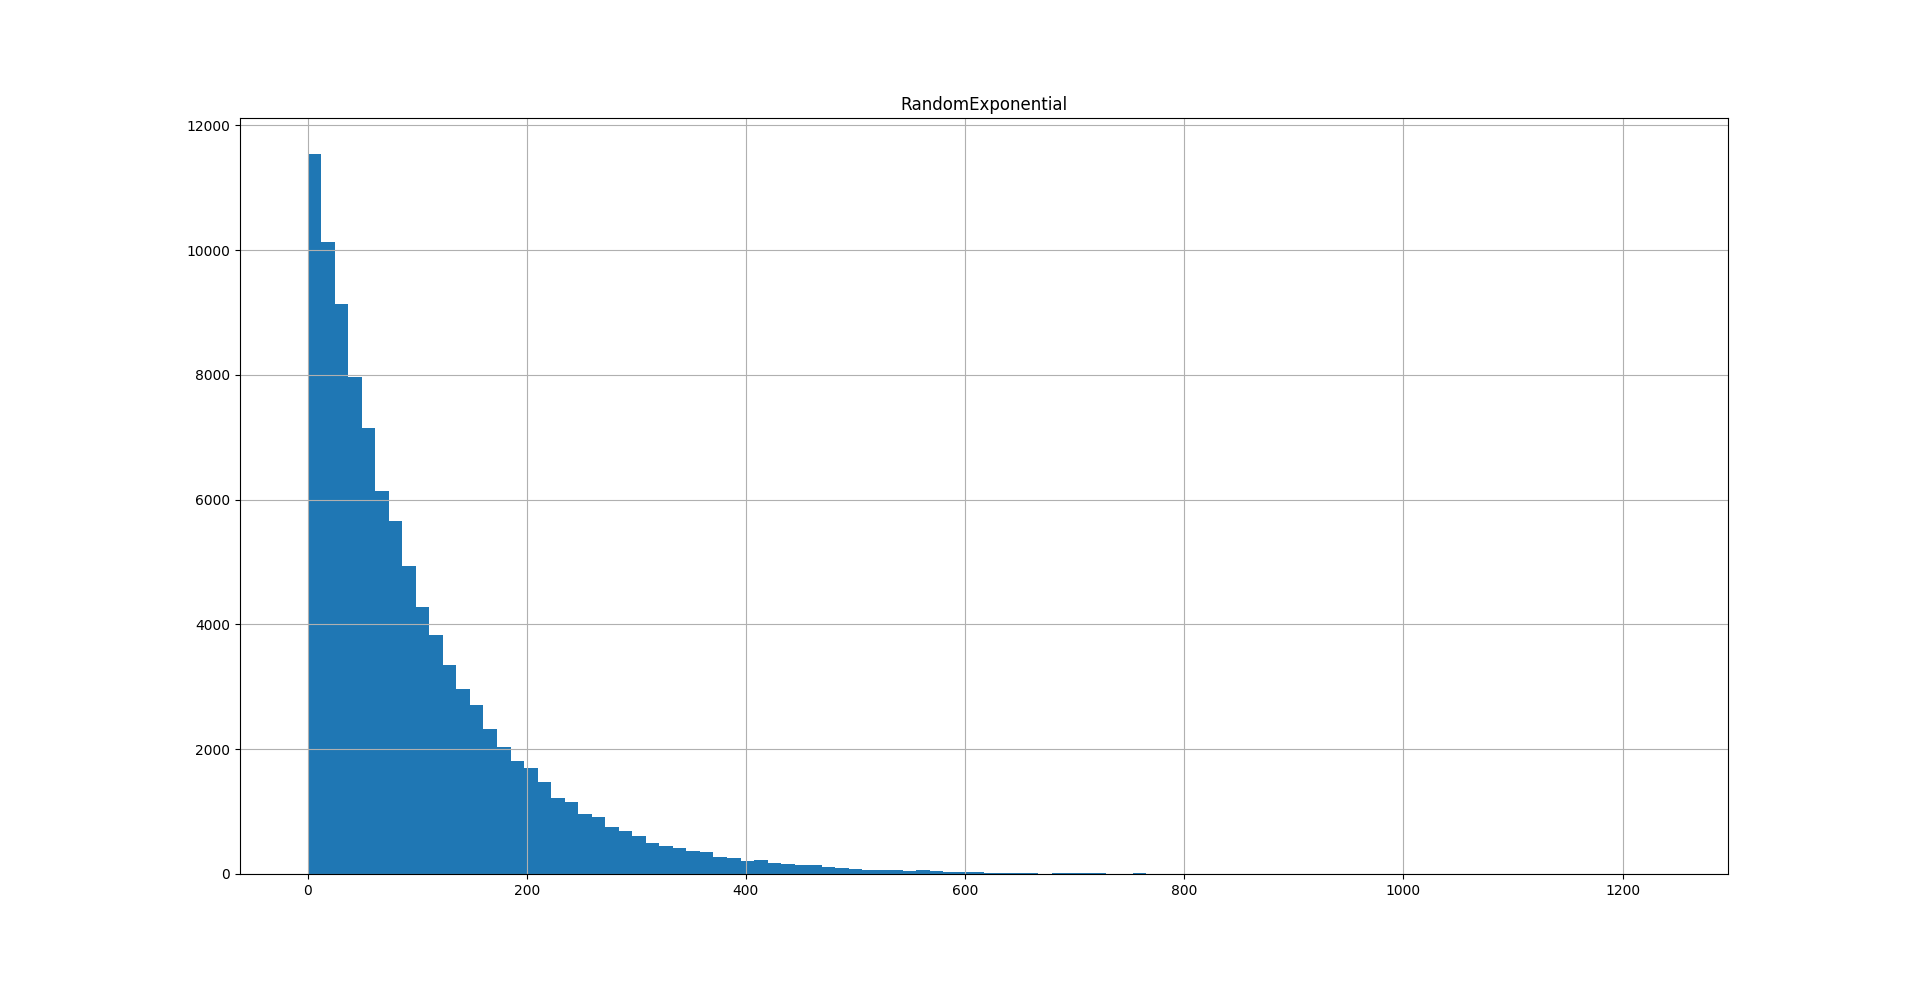
\includegraphics[width=\linewidth]{ns3exponential.png}
      \caption{ns-3 RandomExponentialVariable implementation.}
      \label{fig:ns-3rev}
  \end{figure}

  \begin{figure}[h!]
    \centering
      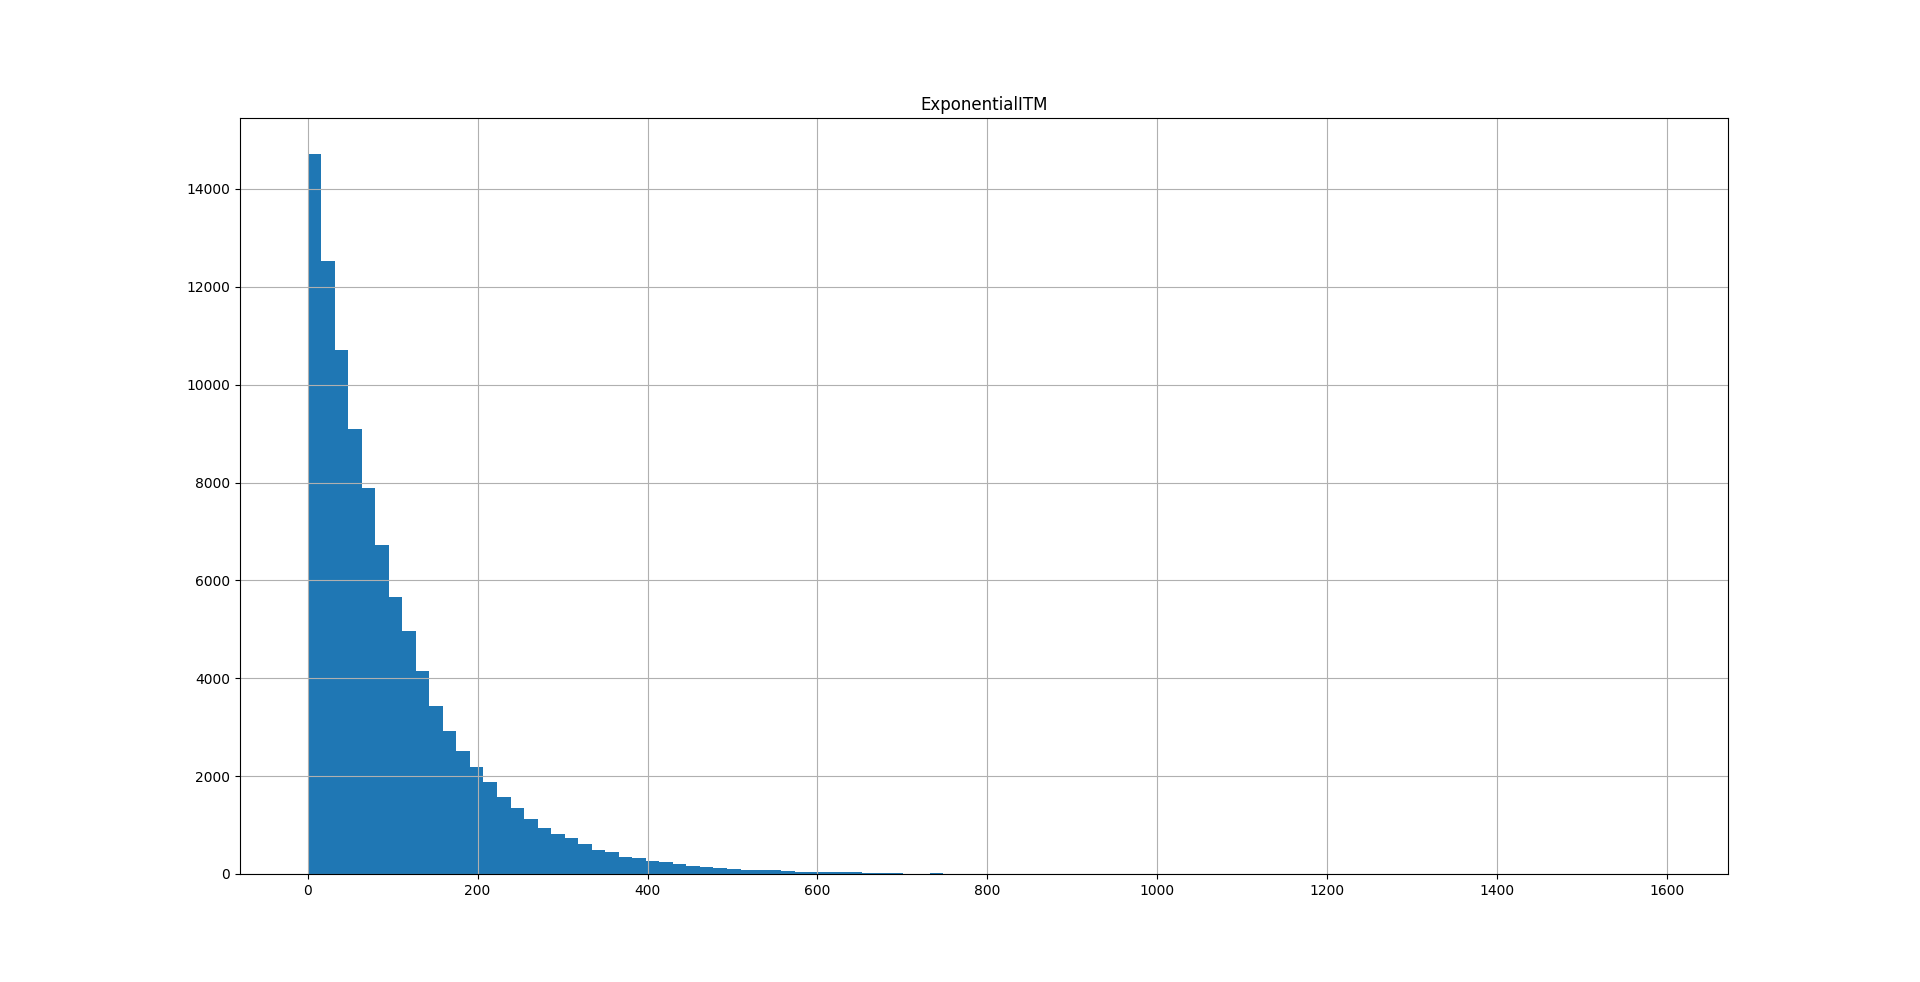
\includegraphics[width=\linewidth]{exponentialITM.png}
      \caption{ITM exponential random variable.}
      \label{fig:itmrev}
  \end{figure}
  \newpage
  
  Figure \ref{fig:itmrev} below shows the distribution achieved when we used ITM to get random exponential variables. 
  There is a small difference here, our implementation has a steeper slope compared to the ns-3 implementation.
  \newpage
  \subsection{Conclusions}
The conclusions from the part 1 of the paper is that we successfully implemented our own random number generator but we
have to be careful choosing the attributes to the generator so that we don't get cycles early and avoid the zero-problem, 
we proved that the Inverse Transform Method works mathematically and showed the ITM that we used for our generation 
of exponential random values. We successfully uncovered how ns-3 gets its normal random numbers by the rejection method
Box-Muller. Finally we compared our exponential random generator to the one in ns-3. Our implementation gave a steeper
slope in the plotted graph compared to the one in ns-3. This might be due to the difference in spread of the uniform
random values. The difference in the plotted graphs for uniform random variables displays a similar shape with little to
no difference.
\newpage
\section{Part II: Mathematical Modelling of a system of Queues} \label{part2}
\begin{figure}[h!]
  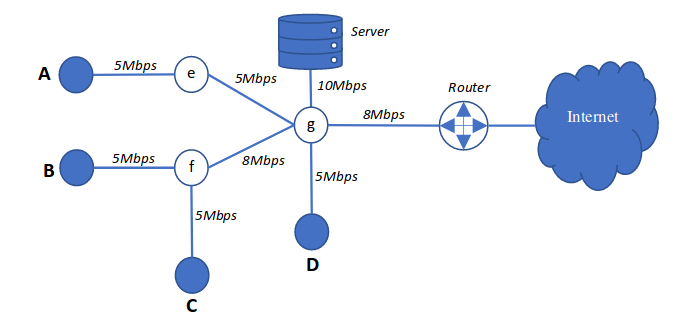
\includegraphics[width=\linewidth]{netmap.png}
  \caption{Network topology}
  \label{fig:netmap}
\end{figure}
By inspecting the figure \ref{fig:netmap} we made a Kleinrock approximation to calculate the average number of 
packets in the system. Kleinrock independence approximation assumes that when you have a dense network of queues
the effects of packet streams going into each other results in independent packet arrival-rates as the speed a packet traverses a line is only dependent on the available bandwidth of that line and how congested it is, then each
queue can be observed as its own M/M/1 system and be observed isolated from each other. Which simplifies calculations
for the whole system. However its still important to remember that it is still just an approximation and might not
represent reality accurately but there is proof that it is still a very good approximation that is worth doing. \cite{kenyon2002high}
\begin{table}[h]
\centering
\label{Arrivalrates}
\caption{Arrival rates}
\begin{tabular}{|l|l|l|}
\hline
$\lambda_{ij}$ & Calculation & Arrival rate (Packets/s) \\ \hline
$\lambda_{ae}$ & $\frac{1}{2ms}$  & 500 \\ \hline
$\lambda_{bf}$ & $\frac{1}{2ms}$  & 500 \\ \hline
$\lambda_{cf}$ & $\frac{1}{0.5ms}$  & 2000 \\ \hline
$\lambda_{dg}$ & $\frac{1}{1ms}$  & 1000 \\ \hline
$\lambda_{fg}$ & $\lambda_{bf} + \lambda_{cf}$  & 2500  \\ \hline
$\lambda_{eg}$ & $\lambda_{ae}$ & 500 \\ \hline
$\lambda_{gs}$ & $\lambda_{fg} + \lambda_{dg} + \lambda_{eg}$ & 4000 \\ \hline
\end{tabular}
\end{table}
We then calculated the arrival-rate based on the inter-arrival times and present them in table \ref{Arrivalrates}. We then calculated the service-rates which were based on the available bandwidth on the channel between each node. These were then presented in table \ref{departurerates}.
\begin{table}[h]
\centering
\label{departurerates}
\caption{Departure-rates}
\begin{tabular}{|l|l|}
\hline
$\mu_{ij}$ & Service-rate(Packets/s)\\ \hline
$\mu_{ae}$ & 6250 \\ \hline
$\mu_{eg}$ & 6250 \\ \hline
$\mu_{bf}$ & 6250 \\ \hline
$\mu_{cf}$ & 6250 \\ \hline
$\mu_{dg}$ & 6250 \\ \hline
$\mu_{fg}$ & 10000 \\ \hline
$\mu_{gs}$ & 12500 \\ \hline
\end{tabular}
\end{table}
The values presented in the tables \ref{Arrivalrates} and \ref{departurerates} were then inserted into the
formula below to calculate the number of packets on each link:
$$N_{ij} = \frac{\lambda_{ij}}{\mu_{ij} - \lambda_{ij} }$$
With the values this becomes the equation-set 1 below:
$$N_{ae} = \frac{\lambda_{ae}}{\mu_{ae} - \lambda_{ae} } \implies \frac{500}{6250 - 500 } = 0.0869565 $$
$$N_{eg} = \frac{\lambda_{eg}}{\mu_{eg} - \lambda_{eg} } \implies \frac{500}{6250 - 500 } = 0.0869565 $$
$$N_{bf} = \frac{\lambda_{bf}}{\mu_{bf} - \lambda_{bf} } \implies \frac{500}{6250 - 500 } = 0.0869565 $$
$$N_{cf} = \frac{\lambda_{cf}}{\mu_{cf} - \lambda_{cf} } \implies \frac{2000}{6250 - 2000 } = 0.470588 $$
$$N_{dg} = \frac{\lambda_{dg}}{\mu_{dg} - \lambda_{dg} } \implies \frac{1000}{6250 - 1000 } = 0.190476 $$
$$N_{fg} = \frac{\lambda_{fg}}{\mu_{fg} - \lambda_{fg} } \implies \frac{2500}{10000 - 2500 } = 0.333333 $$
$$N_{gs} = \frac{\lambda_{gs}}{\mu_{gs} - \lambda_{gs} } \implies \frac{4000}{12500 - 4000 } = 0.470588 $$
$$Equations\ 1.\ Individual\ number\ of\ packets.$$

Later we used the formula below to calculate the average number of packets in the whole system:
$$ \overline{N} = \sum N_{ij} $$
Which gave us the resulting equation-chain:
$$ \overline{N} = \sum N_{ij} = \frac{500}{6250 - 500 } + \frac{500}{6250 - 500 } + \frac{500}{6250 - 500 } + \frac{2000}{6250 - 2000 } + $$ 
$$ \frac{1000}{6250 - 1000 } + \frac{2500}{10000 - 2500 } + \frac{4000}{12500 - 4000 } = 1.638898 packets $$ 


Which concludes the section with the answers to the questions on part 2. The average number of packets are 1.638898
packets and the number of packets per link can be found in equations 1.


\newpage
\section{Part III: Simulations and Results Comparison} \label{part3}

\subsection{Implementation}
We decided to use the ns-3 discrete event network simulator to implement and test the proposed scenario.



\subsubsection{Network topology}
Our network topology consisting of ns-3-nodecontainers were interconnected using a point-to
-point helper. The point-to-point helper was used to set the queue-type for all of the
nodes in the network and set the type of queue for all of them. The resulting configuration
for it was five Mbit/s links, two eight Mbit/s links and a ten Mbit/s link where all of
them had a single-server, drop-tail queue. We assumed a infinite queue so this attribute
didn't do much. 

Following this we installed a internet-stack-helper to help with the stack, a
trafic-control-helper to set the queuing discipline and a Ipv4-address-helper to give each
node an ip. 

Lastly we installed the server- and router-applications where the server was a modified
udp-echo-server and the router was a packet-sink which would discard all packets it
received. 

The topology for the csma version is very similar to the point-to-point version. The only
difference is that the point-to-point-helper was changed to a csma-helper where it got the
same bandwidth values and queue types as the previous version. However this change turned
the channels into half-duplex channels instead of full-duplex as they were previously. This
is due to that they now share a bus to transfer over and if both sides transmit at the same
time, the packets will collide and be dropped.


\subsubsection{Server implementation}
To get the desired behaviour where the server only replies to 70\% of messages and 30\% are sent to the router.
We decided to implement our own version of the UdpEchoServerHelper and UdpEchoServer application.
The new versions of theses classes were called MyUdpEchoServerHelper and MyUdpEchoServer.
When implementing the behaviour first all code in UdpEchoServerHelper and UdpEchoServer was copied into MyUdpEchoServerHelper and MyUdpEchoServer respectively.
We then modified the behaviour by adding the router address as a parameter into the helper class constructor.
This address was stored in a private member variable called m\_routerAddress.
This address needed to be sent to the MyUdpEchoServer application that the helper creates.
So in the private install function of the helper class we use the object factory to create a pointer to a MyUdpEchoServer object then the router address is set in this object by calling a setter function.
The application is then added to the node that the helper is installing.

The modifications made to the MyUdpEchoServer class is first that two private member variables were added one for the
router address called m\_routerAddress and one pointer for the uniform random variable called randVar.
The router address is set by the helper using a setter function and the random variable is set in the class constructor using the create object function.
To change the behaviour the only other function that needed modification was HandleRead.
In this function we first generate a random variable using the uniform random variable.
Then if the value is larger then 0.7 a bool is set to true.
This bool variable decides if the message should go to the router or not.
When the response packet is sent the bool variable is checked and the router address i applied if true and the sender address is applied if false.

We were able to place the two classes MyUdpEchoServer and MyUdpEchoHelper in a sub folder within our project directory.
The reason to place the classes in a sub folder is because the waf program only checks for .cc files two folders deep in the scratch folder.
To get the two class files to compile we needed to register the relative path for them in the src/application/model and src/application/helper folders.
This could be done by editing the wscript file in the src/application folder.
Then when rebuilding ns-3 our classes appeared as regular application classes.

\subsubsection{Scheduling}
To schedule sending events for the different sending node A, B, C and D the simulator function called ScheduleWithContext was used.
This function takes a callback function that generates new data by first randomizing the packet size with an exponential random variable and then sending the packet.
After the packet is sent a new call to the traffic generator function is scheduled using the simulator's ScheduleWithContext.
The time to the next packet is set to follow an exponential random variable.
This results in the nodes sending packets according to a Poisson process.
This means that none of the sending nodes have any applications installed instead the sending behaviour is directly handled by the simulator.
First we considered using an OnOffHelper to send packets where the off time was exponentially distributed but we could not find any way to make it use our random number generator.
We also considered creating our own version of the UdpEchoClient application but this would be much more time consuming than just directly handling the packet sending with the simulator, which is what we decided to use.

\subsubsection{Logging method}
The type of data we wanted to be able to see when logging was the queue lengths for each connection and delay for each flow of data.
We also used pcap to log the packets for some nodes for debugging purposes.

To log the number of packets that were in each queue we used the simulator to schedule calls to a logging function.
This function took as parameters the queue container that keeps the status for each queue as well as a file stream.
The number of packets in each queue was then logged as comma separated values which made it very easy to take the outputted file and do analysis on it using python.

To get information on the delay values of each flow of data we used the ns-3 flow monitor tool to output an XML containing all the flow information.
We could then read that file and see the total delay for all flows.
This could then be used to calculate the average delay on a specific link.

\subsection{Simulation}
When simulating the final setup we compared it to the calculated expectations. For the average 
number of packets between node G and the server was calculated to be around 0.47 packets, 
however the simulated result was around 0.064 packets which is significantly smaller than the 
expected calculation deems. 

The average queuing delay and total average delay for the packets traversing the link F to G 
was acquired by creating a flow-monitor statistical analyser file. From that resulting XML-file 
we calculated the delay by taking the delaysum for the flow. We used the total delay values for 
the nodes that is presented just below.
$$\frac{((b \rightarrow g) - (b \rightarrow f)) + ((c \rightarrow g) - (c \rightarrow f))}{number\ of\ packets}$$
Which resulted with the delay from F to G to be about 0.123 milliseconds.  
When observing the delay between A and the server we got that it was around 0.454 milliseconds 
and the reversed path (server to A) was around 0.478 milliseconds. 

Later we changed the point-to-point configuration to a CSMA-based one. This had change did not 
have any significant effect on the data rate or the delay as the differences were negligible.
However the number of packets in queue at the server to G queue was huge.

Finally we swapped the NS-3 random variables to our implemented versions. When we did this we
barely noticed any difference. We almost got the same results as before except abit lower.
The queue size form G to server was now 0.055.
The delay between F and G was now about 0.121 milliseconds.
The Delay from F to G was unchanged, the delay from the server to A was 0.46 which is slightly 
lower than before and from A to the server was now 0.48 . These are however within the bounds 
of deviations so we can say that they are equal.

\newpage
\subsubsection{Results}
\begin{figure}[!htbp]
    \centering
    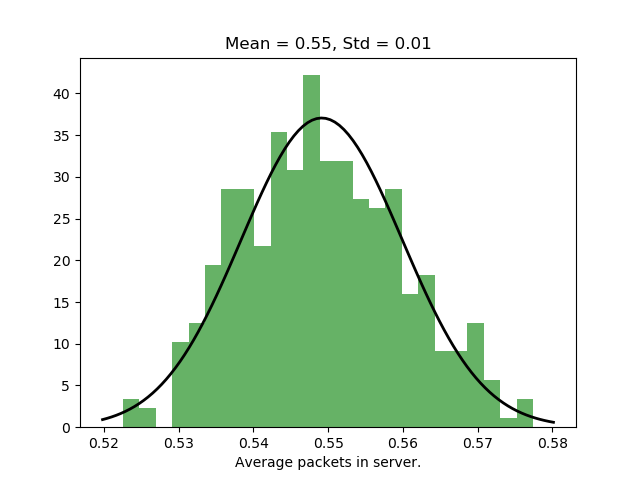
\includegraphics[width=0.85\linewidth]{ns3_gs_queue_size.png}
    \caption{The number of packets from g to the server using ns3's random number implementation.}
    \label{fig:GtoServerNs3}
\end{figure}

Figure \ref{fig:GtoServerNs3} shows the average number of packets in queue from g to the server when using ns3's random number implementation.
The actual value is with 95\% confidence $0.549 \pm 0.00115$.
The value was simulated by sampling the queue sizes at different times and taking the average value from that.
Then to get the average number of packets under service in the server we took the total delay for all flows going from the server through g and divided that by the total running time.
To get the result shown in figure \ref{fig:GtoServerNs3}, 400 simulations were done.


\begin{figure}[!htbp]
    \centering
    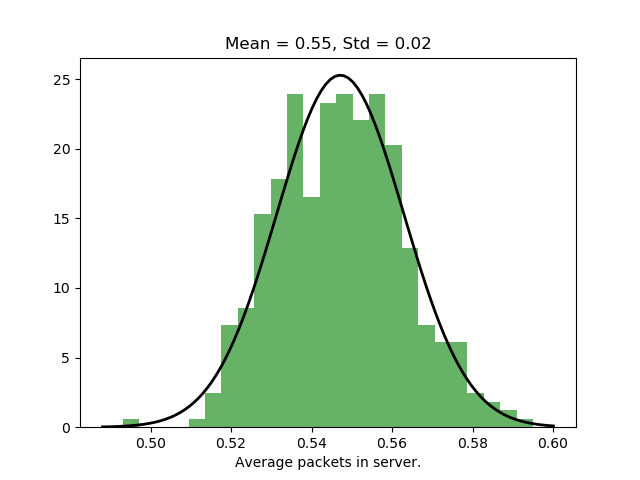
\includegraphics[width=0.85\linewidth]{our_gs_queue_size.png}
    \caption{The number of packets from g to the server using our random number implementation.}
    \label{fig:GtoServerOur}
\end{figure}

Figure \ref{fig:GtoServerOur} shows the average number of packets in queue from g to the server when using our random number implementation.
The actual value is with 95\% confidence $0.547 \pm 0.001680$.
The value was simulated in the same way as for the ns3 results the only difference was the random number generator used.
To get the results shown in figure \ref{fig:GtoServerOur}, 400 simulations were done.

\begin{figure}[!htbp]
    \centering
    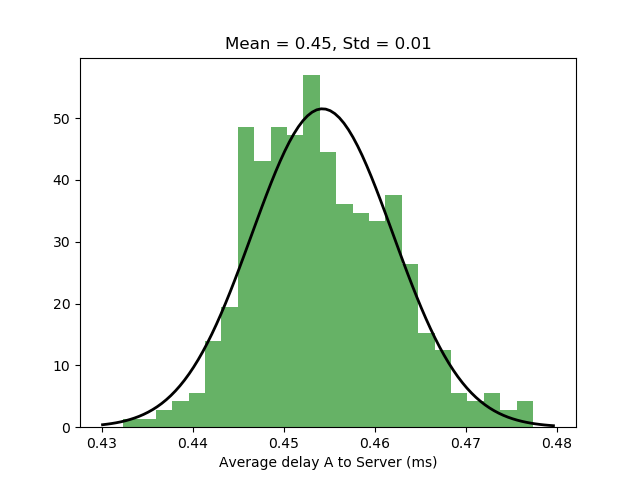
\includegraphics[width=0.85\linewidth]{ns3_as_delay.png}
    \caption{The average delay for packets going from a to the server using the ns3 random number implementation.}
    \label{fig:AtoServerNs3}
\end{figure}

Figure \ref{fig:AtoServerNs3} shows the average delay for packets going from A to the server when using the ns3 random number implementation.
The actual value is with 95\% confidence $0.454 \pm 0.00426$ milliseconds.
The value was simulated by checking the total delay of the A to server flow and dividing that by the number of packets traversing that flow.
To get the results shown in figure \ref{fig:AtoServerNs3}, 400 simulations were done.

\begin{figure}[!htbp]
    \centering
    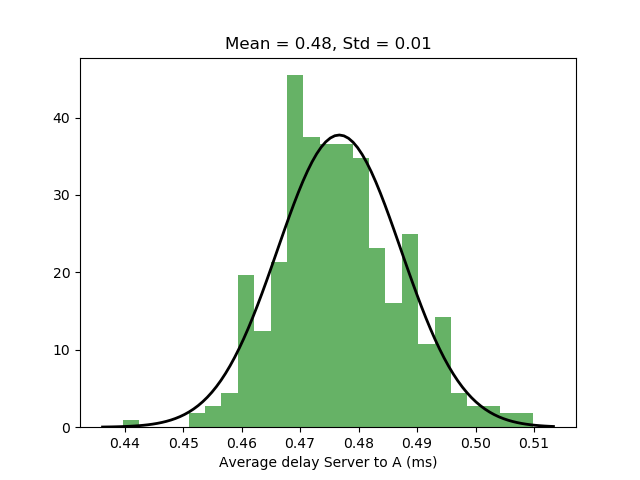
\includegraphics[width=0.85\linewidth]{ns3_sa_delay.png}
    \caption{The average delay for packets going from the server to A using the ns3 random number implementation.}
    \label{fig:ServerToANs3}
\end{figure}

Figure \ref{fig:ServerToANs3} shows the average delay for packets going from the server to A when using the ns3 random number implementation.
The actual value is with 95\% confidence $0.477 \pm 0.00582$ milliseconds.
The simulated value was obtained in the same way as the simulated value from A to the server.
To get the results shown in figure \ref{fig:ServerToANs3}, 400 simulations were done.

\begin{figure}[!htbp]
    \centering
    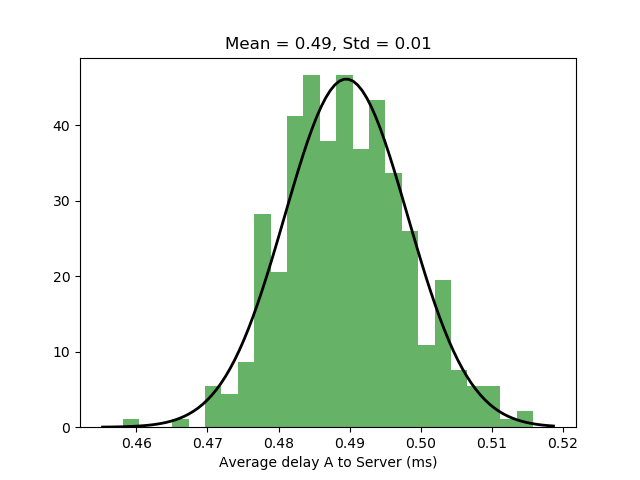
\includegraphics[width=0.85\linewidth]{our_as_delay.png}
    \caption{The average delay for packets going from A to the server using our random number implementation.}
    \label{fig:AtoServerOur}
\end{figure}

Figure \ref{fig:AtoServerOur} shows the average delay for packets going from A to the server when using our random number implementation.
The actual value is with 95\% confidence $0.490 \pm 0.00476$ milliseconds.
The simulated value was obtained in the same way as the corresponding ns3 value.
To get the results shown in figure \ref{fig:AtoServerOur}, 400 simulations were done.

\begin{figure}[!htbp]
    \centering
    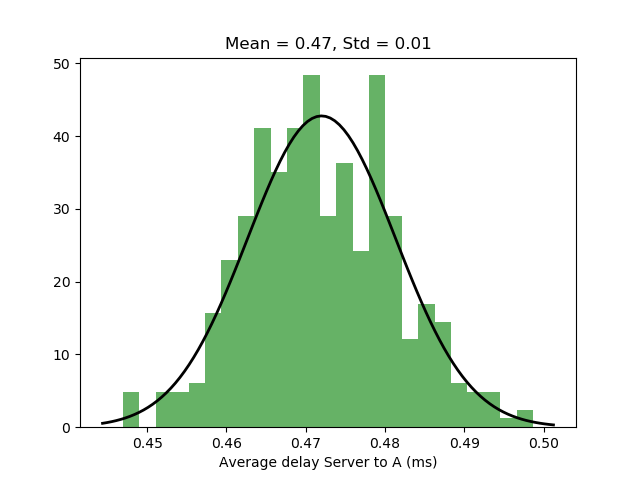
\includegraphics[width=0.85\linewidth]{our_sa_delay.png}
    \caption{The average delay for packets going from the server to A using our random number implementation.}
    \label{fig:ServerToAOur}
\end{figure}

Figure \ref{fig:ServerToAOur} shows the average delay for packets going from the server to A when using our random number implementation.
The actual value is with 95\% confidence $0.472 \pm 0.005130$ milliseconds.
The simulated value was obtained in the same way as the corresponding ns3 value.
To get the results shown in figure \ref{fig:ServerToAOur}, 400 simulations were done.


\begin{figure}[!htbp]
    \centering
    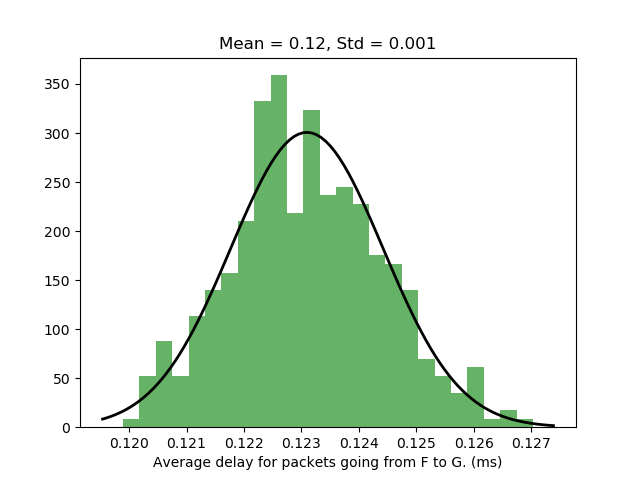
\includegraphics[width=0.85\linewidth]{ns3_fg_delay.png}
    \caption{The average delay for packets going from F to G when using the ns3 random number implementation.}
    \label{fig:FGNs3}
\end{figure}

Figure \ref{fig:FGNs3} shows the average delay for packets going from F to G when using the ns3 random number implementation.
The actual value is with 95\% confidence $0.123 \pm 0.00073$ milliseconds.
The simulated value was obtained by measuring the delay for B and C flows to G and then subtracting the delay for B and C to F.
This gives the total delay for that connection, so to get the average delay the total value is divided by the number of packets.
$$\frac{((b \rightarrow g) - (b \rightarrow f)) + ((c \rightarrow g) - (c \rightarrow f))}{number\ of\ packets}$$
To get the results shown in figure \ref{fig:FGNs3}, 400 simulations were done.

\begin{figure}[!htbp]
    \centering
    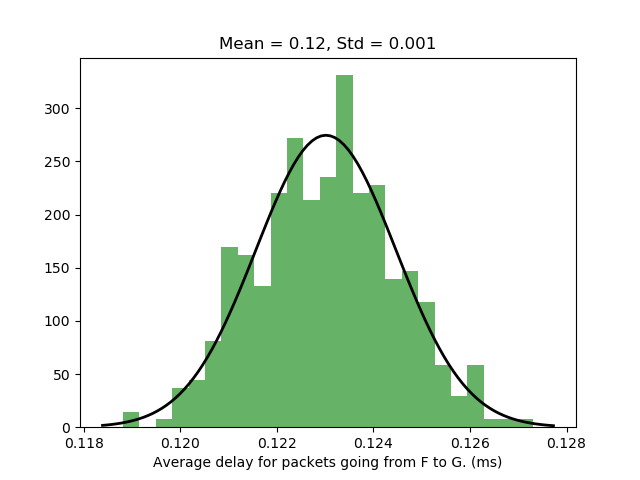
\includegraphics[width=0.85\linewidth]{our_fg_delay.png}
    \caption{The average delay for packets going from F to G when using our random number implementation.}
    \label{fig:FGOur}
\end{figure}

Figure \ref{fig:FGOur} shows the average delay for packets going from F to G when using our random number implementation.
The actual value is with 95\% confidence $0.123 \pm 0.00080$ milliseconds.
The simulated value was obtained in the same way as the corresponding ns3 value.
To get the results shown in figure \ref{fig:FGOur}, 400 simulations were done.

\begin{figure}[!htbp]
  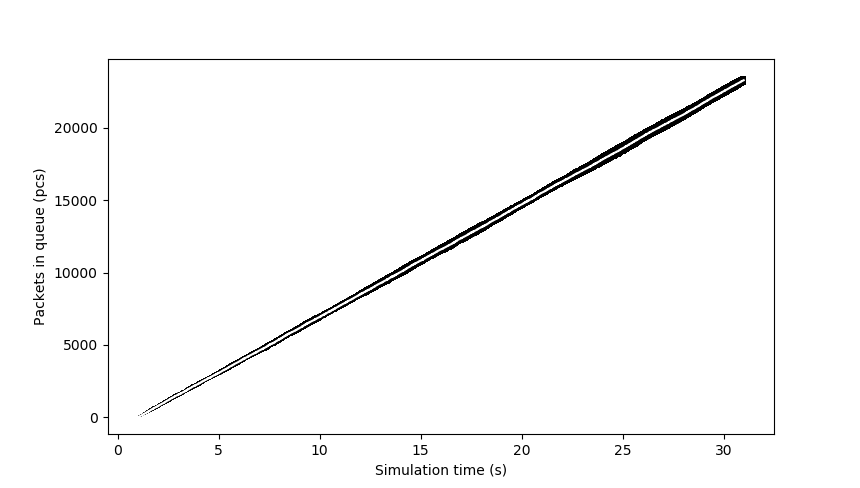
\includegraphics[width=\linewidth]{queuecsma.png}
  \caption{Queuelength at the server when using CSMA.}
  \label{fig:csmaqueuelen}
\end{figure}
Figure \ref{fig:csmaqueuelen} shows the increasing queue length at the server when using busses and csma instead of point to point connections. The white line is the mean of 15 measurements and the black area around it is the standard deviation of these 15 measurements. It demonstrates the ever increasing queue-size as more and more packets become backlogged.

\subsubsection{Evaluation}
The difference in number of packets between G and the server is of a noticeable size. We have 
two theories around why that is the case.

\textbf{First} the calculations use the Kleinrock independence approximation which may not be 
a good approximation for the system. This is because the system has quite low traffic while the 
Kleinrock approximation works better for high traffic systems. We tested halving all the data 
rates in the system and got results more close to the calculated values.

\textbf{Second} the simulation might not take into account the packets that are in service 
by only counting the packets that are in queue. This might be responsible for part of the 
error since the Kleinrock approximation calculates the total number of packets in the point 
to point connection. When measuring the average queue size between g and the router the 
results are 0.This is probably because the router is able to consume the packet fast enough 
so that no queue has time to form.

When we changed to CSMA on busses we got a larger queue at the server to G. This is probably due
to the fact that we have the combined transmissions from G redirected from D, E and F which are 
all heading to the server, which the return packets has to fight for space against. And since the
busses are only half-duplex and can only send in one direction at a time there will be packet 
collisions on that bus, which adds more and more packets at the server to G backlog for re-transmissions.
This is represented in the image below where the large packet streams are heading towards G and a bunch 
of slower responses are heading back from the server which they have to fight for space against, which 
leads to a backlog forming at G for the responses.
\begin{figure}[h!]
  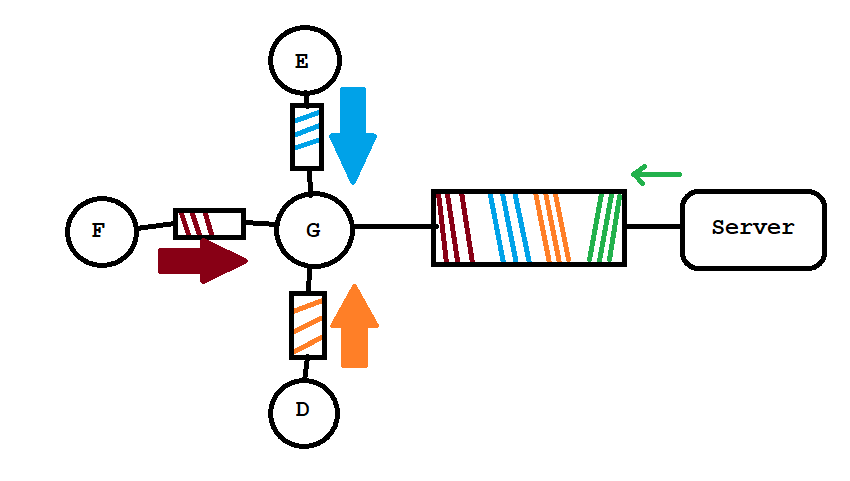
\includegraphics[width=\linewidth]{csmamap.png}
  \caption{CSMA flow map}
  \label{fig:csma}
\end{figure}
\newpage
\subsection{Conclusions}
The implementation of the network topology was quite straight forward especially since only point to point connections had to be used.
The implementation of the server behaviour did however require a bit of research on our part.
This was mainly because we used git as a version control tool and in the beginning we thought that our own class implementation files had to be put into the ns-3 source directory for it to be compiled.
Eventually we found that by modifying some of the building script we could put the class files in our project directory.
For scheduling the way we decided to implement it was good since we planed on replacing the random variables from ns-3's implementation to our own implementation.
So working directly with the simulator scheduling functions was a good idea.
When implementing we found it very useful to be able to log pcap files so that we could monitor the packet traffic for specific nodes.

\bibliographystyle{unsrt}
\bibliography{ref}
\end{document}
